%!TEX TS-program = pdflatex
\documentclass{robinthesis}
\tikzstyle{every picture}+=[remember picture, >=latex]

\begin{thesischapter}{Coh}{Some Coherence Results}
%
In this chapter, we prove some new coherence results for
Gray monoids. These results pave the way for the following
chapter, which describes a simple but apparently novel
technique for stating definitions and performing calculations
in a monoidal bicategory.

At the time of writing, the sum of human knowledge about
coherence for monoidal bicategories -- and, more generally, for
tricategories -- is contained in the PhD dissertation of
\citet{GurskiThesis}, which builds on the pioneering work
of \citet{GPS}. Nothing has yet been written about coherence
for \emph{braided} monoidal bicategories. It is gradually
becoming clear that tricategories, and other such higher-dimensional
structures, enjoy more coherence than they are generally credited with.
One manifestation of this is that many diagrams of 2-cells commute
in any Gray monoid. To be precise, we shall prove:
\begin{thm}\label{thm-coh}
	In the free Gray monoid generated by a multigraph,
	every diagram of 2-cells commutes.
\end{thm}
This strengthens Gurski's Theorem~10.2.2, which (specialised to
monoidal bicategories) addresses the free Gray monoid generated
by a mere graph, rather than a multigraph. It is apparently possible
to strengthen it still further, but the statement here is
adequate for our present purposes.

Our second result encompasses the braided case:
\begin{thm}\label{thm-coh-braiding}
	In the free braided Gray monoid generated by
	a multigraph, every diagram of 2-cells whose
	source and target are `positive' 1-cells commutes.
\end{thm}
Here `positive' means that the 1-cell is built without using
$s'$, the equivalence inverse of $s$. This restriction is made
because it significantly simplifies the proof, yet remains sufficient
for our applications in this work. The result does appear in fact
to hold for all 2-cells, and we conjecture that a more complex
application of the techniques of this chapter suffices to prove
the general version.

In both cases, the method of proof is essentially that used
by \citet{MacLane} in his coherence theorem for monoidal categories,
using term rewriting. This syntactic technique seems
to permit a finer analysis of coherence than the
powerful but blunt semantic methods employed by \citet{GPS}
and refined by \citet{GurskiThesis}.

\section{Non-braided Case}
A multigraph consists of the data for a multicategory, but
without the identity arrows or the composition operation.
More formally,
%\begin{definition}\label{def-multigraph}
	a multigraph $G$ consists of:
	\begin{itemize}
		\item a set $G_{0}$ of objects,
		\item for each finite `source' sequence $A_{1}, \dots, A_{n}$
			of objects and `target' object $B$, a set $G(A_{1},\dots,A_{n}; B)$
			of multiarrows.
	\end{itemize}
%\end{definition}
% The above definition is in `enriched' style; alternatively,
% in `internal' style, a multigraph is a span
% \begin{diagram}[vtriangleheight=2em]
%	&&G_{1} \\
%	&\ldTo^{s} && \rdTo^{t} \\
%	G_{0}^{*} &&&& G_{0}
% \end{diagram}
% of sets, where of course $(-)^{*}$ denotes the free monoid functor.
% The latter style of definition permits a marginally tidier definition
% of the morphisms of multigraphs: if $G$ and $H$ are multigraphs,
% a morphism $f: G\to H$ consists of functions $f_{0}: G_{0}\to H_{0}$
% and $f_{1}: G_{1}\to H_{1}$ such that the diagram
% \begin{diagram}[w=2em]
%	&&G_{1} \\
%	&\ldTo^{s} &\dTo>{f_{1}}& \rdTo^{t} \\
%	G_{0}^{*} &&H_{1}&& G_{0} \\
%	\dTo<{f_{0}^{*}} &\ldTo_{s}&& \rdTo_{t} & \dTo>{f_{0}} \\
%	H_{0}^{*} &&&& H_{0}
% \end{diagram}
% commutes. In the enriched style,
A morphism of multigraphs
$f: G\to H$ consists of an object function $f_{0}: G_{0}\to H_{0}$ 
together with a family of functions
\[
	f_{A_{1},\dots,A_{n};B}: G(A_{1},\dots,A_{n};B) \to H(f_{0}(A_{1}),\dots,f_{0}(A_{n});f_{0}(B)).
\]
The category $\cat{GrayMon}_\mathrm{str}$ of Gray monoids and \emph{strictly} structure-preserving
maps has an obvious forgetful functor to the category of multigraphs, and clearly this forgetful functor can be furnished with a left adjoint $F$ by the usual syntactic construction. Naively, then, the objects,
1-cells and 2-cells of the Gray category $F(G)$ are formal expressions built from the objects and
multiarrows of $G$, quotiented by the smallest equivalence relation that makes the resulting
structure into a Gray monoid, i.e. the equivalence relation generated by the axioms that define
Gray monoid. But of course this description can be simplified, as follows.

Since the objects of a Gray monoid form a monoid under tensor, an object of $F(G)$ can be represented
by a finite sequence $\tuple{X_{1},\dots,X_{n}}$ of objects of $G$;
the tensor of two objects is their concatenation as sequences, and
the unit object is represented by the empty sequence.
%
Turning next to the 1-cells, notice that since the tensor of $f: A\to B$ and $g: C\to D$
is equal to $(B\tn g)(f\tn C)$, the tensor of 1-cells can be expressed in terms of
the tensor of a 1-cell with an object, and composition. Therefore we need
not regard the tensor of two 1-cells as a primitive operation, provided that we can
take the tensor of a 1-cell with an object.
%
Furthermore, every 1-cell is equal to a finite composite of \emph{multiarrow 1-cells},
where a multiarrow 1-cell is obtained by tensoring a multiarrow of $G$ with objects, on
either side. More formally, a multiarrow 1-cell
\[
	\langle X_{1},\dots,X_{m}\rangle \to \langle Y_{1},\dots,Y_{n}\rangle
\]
consists of a natural number $1\leq j\leq n$ and a multiarrow
\[
	f \in G(X_{j},\dots,X_{j+m-n}; Y_{j})
\]
such that $\langle X_{1}, \dots, X_{j-1}\rangle = \langle Y_{1}, \dots, Y_{j-1}\rangle$
and $\langle X_{j+m-n+1}, \dots, X_{m}\rangle = \langle Y_{j+1},\dots, Y_{n}\rangle$.
This might be pictured as follows:
\[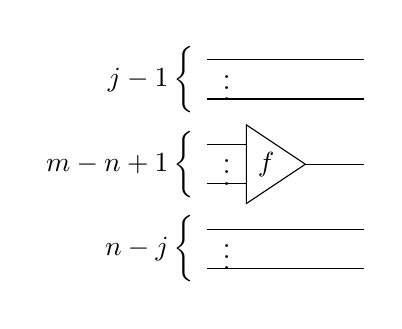
\begin{tikzpicture}
	\newcommand\wires[1]{
		\begin{scope}
			\pgftransformscale{0.25}
			\node[left] at (0,0) {
				$#1
				\left\{\hbox{\vrule height 8pt depth 8pt width 0pt}\right.$
			} ;
			\draw (0,1) -- +(8,0) ;
			\node at (1,0) {\vdots} ;
			\draw (0,-1) -- +(8,0) ;
		\end{scope}
	}
	\newcommand\multiarrow[2]{
		\begin{scope}
			\pgftransformscale{0.25}
			\node[left] at (0,0) {
				$#1
				\left\{\hbox{\vrule height 8pt depth 8pt width 0pt}\right.$
			} ;
			\draw (0,1) -- +(2,0) ;
			\node at (1,0) {\vdots} ;
			\draw (0,-1) -- +(2,0) ;
			\draw (2,-2) -- ++(0,4) -- ++(3,-2) -- cycle ;
				\node at (3,0) {$#2$} ;
			\draw (5,0) -- ++(3,0) ;
		\end{scope}
	}
	\matrix {
		\wires{j-1} \\ \multiarrow{m-n+1}{f} \\ \wires{n-j} \\
	} ;
\end{tikzpicture}\]
Similarly, the tensor of 2-cells can be expressed in terms of
the tensor of a 1-cell with an object, and horizontal composition.
In turn, horizontal composition can be expressed in terms of whiskering
and vertical composition. Therefore our 2-cells may be built from
\emph{interchange cells}, where an interchange cell is either
a \emph{positive interchange cell} $b_{\vec X,f,\vec Y,g,\vec Z}$ like this:
\[
	\newcommand\tube[1]{
		\draw[double] node[left] {$#1\phantom{\scriptstyle1}$} (0,0) -- +(12,0) ;
	}
	\newcommand\multiarrow[5][2]{
		\draw (0, 1) node[left] {$#2_{1}$} -- +(#1,0) ;
		\node at (1,0) {\vdots} ;
		\draw (0,-1) node[left] {$#2_{\rlap{$\scriptstyle #3$}\phantom{1}}$} -- +(#1,0) ;
		\draw (#1,-2) -- ++(0,4) -- ++(3,-2) -- cycle ;
			\node at (1+#1,0) {$#4$} ;
		\draw (3+#1,0) -- (12,0) node[right] {$#5$} ;
	}
	\tikzstyle{every picture}+=[baseline]
	\tikzstyle{every cell}	 +=[scale=0.25]
	\begin{tikzpicture}
	\matrix {
		\tube{\vec X} \\
		\multiarrow{A}{m}{f}{B} \\
		\tube{\vec Y} \\
		\multiarrow[8]{C}{n}{g}{D} \\
		\tube{\vec Z} \\
	} ;
	\end{tikzpicture}
	\quad \To \quad
	\begin{tikzpicture}
	\matrix {
		\tube{\vec X} \\
		\multiarrow[8]{A}{m}{f}{B} \\
		\tube{\vec Y} \\
		\multiarrow{C}{n}{g}{D} \\
		\tube{\vec Z} \\
	} ;
	\end{tikzpicture}
\]
or a \emph{negative interchange cell} $b_{\vec X,f,\vec Y,g,\vec Z}^{-1}$ in
the other direction. In case it is not clear from the picture, a positive
interchange cell is a 2-cell
\[
  b_{\vec X,f,\vec Y,g,\vec Z}:
	(\vec X\tn B\tn\vec Y\tn g\tn\vec Z)
	\cdot
	(\vec X\tn f\tn\vec Y\tn\vec C\tn\vec Z)
	\To
	(\vec X\tn f\tn\vec Y\tn D\tn\vec Z),
	\cdot
	(\vec X\tn \vec A\tn\vec Y\tn g\tn\vec Z)
\]
where $f \in G(\vec A;B)$ and $g\in G(\vec C;D)$.
In context, we shall omit some of the subscripts and write just $b_{f,g}$.
Now a \emph{basic 2-cell} is the result of whiskering an interchange cell on both
sides, by arbitrary 1-cells, and every 2-cell is a finite vertical composite
of basic 2-cells.

To summarise, a 1-cell $f$ may be canonically represented as a finite sequence of multiarrow cells.
There is a basic 2-cell $f\To g$ whenever $g$ can be obtained from $f$ by interchanging
two adjacent (but non-interfering) multiarrows. (In particular, $f$ and $g$ contain the
same number of multiarrow cells.)

As explained above, we plan to use Mac Lane's technique for proving coherence.
So the next step is to define a rewriting system on 1-cells,
where each rewrite rule corresponds to a basic 2-cell. We shall
show that this rewriting system is strongly normalising and locally confluent,
hence that every 1-cell is isomorphic to one in normal form. Now, local confluence
means that, for every 1-cell $f$, if we have rewriting steps $\gamma: f \To f_{1}$
and $\delta: f\To f_{2}$ then there are sequences of rewrites $\gamma^{*}: f_{1}\To g$
and $\delta^{*}: f_{2}\To g$ for some 1-cell $g$. The final requirement is to show
that the corresponding diagram of 2-cells commutes:
\begin{diagram}
	f & \rTo^{\gamma} & f_{1} \\
	\dTo<\delta && \dTo>{\gamma^{*}} \\
	f_{2} & \rTo_{\delta^{*}} & g.
\end{diagram}
It will be convenient, of course, to prove this at the same time as we establish
local confluence. This extended confluence property does not seem to have a standard
name: we shall call it \emph{local coherent confluence}. Notice that, in a strongly
normalising system, local coherent confluence implies \emph{(global) coherent confluence}:
i.e. given any \emph{sequences} of rewrites $\gamma: f \To f_{1}$
and $\delta: f\To f_{2}$, there are sequences of rewrites $\gamma^{*}: f_{1}\To g$
and $\delta^{*}: f_{2}\To g$ for some 1-cell $g$ such that the corresponding diagram
of 2-cells commutes.

In this, the non-braided case, the required rewriting system is very simple:
we treat every 1-cell as a composite of multiarrow 1-cells, and a rewriting step
simply corresponds to a positive interchange cell applied to a pair of
consecutive multiarrow 1-cells.
\begin{lemma}
	This rewriting system is strongly normalising, i.e.\ every reduction
	path is finite.
\end{lemma}
\begin{proof}
	We shall define a weighting function that assigns a natural number to each 1-cell,
	so that each rewriting step strictly decreases the weight. The appropriate weighting function
	here is the \emph{total prefix weight}, which is defined as follows. Recall that
	a 1-cell is represented as a sequence $f_{1}, \dots, f_{n}$ of multiarrow 1-cells. If we
	imagine the 1-cell drawn as a diagram like those above, then each output wire (at the
	far right of the diagram, according to our convention above) is attached to a distinct
	tree of multiarrows. Define the \emph{weight} of an output wire to be the number of multiarrows
	in the tree. So for each multiarrow, the weight of its output wire is $1+$ the sum of
	the weights of its input wires.
	
	A multiarrow 1-cell consists of a single multiarrow with a number of bare wires (objects)
	above and below it. Let us refer to the bare wires above as the `prefix' of the multiarrow 1-cell.
	In the context of a 1-cell $f_{1}, \dots, f_{n}$, define the \emph{prefix weight} of a
	constituent multiarrow 1-cell $f_{i}$ to be the sum of the weights of each wire in the prefix.
	For example, in the diagram below each wire is annotated with its weight, and each
	multiarrow is annotated with its prefix weight.
\[
	\def\triangle(#1,#2)#3 ; {
		\draw (#1,#2-2) -- ++(0,4) -- ++(3,-2) -- cycle ;
			\node at (1+#1,#2) {#3} ;
	}
	\tikzstyle{every picture}+=[baseline,scale=0.25]
	\begin{tikzpicture}
		\draw (0,3)	 node[above right] {$\scriptstyle 0$} -- +(4,0) ;
			\triangle (4,3) {$\scriptstyle 0$} ;
			\draw (7,3) node[above right] {$\scriptstyle 1$} -- +(6,0) ;
		\draw (0,0)	 node[above right] {$\scriptstyle 0$} -- +(8,0) ;
		\draw (0,-2) node[above right] {$\scriptstyle 0$} -- +(8,0) ;
			\triangle (8,-1) {$\scriptstyle 1$} ;
			\draw (11,-1) node[above right] {$\scriptstyle 1$} -- +(2,0) ;
		\draw (13,3)  -- ++(2,-1) -- +(2,0) ;
		\draw (13,-1) -- ++(2,1)  -- +(2,0) ;
		\triangle (17,1) {$\scriptstyle 0$} ;
		\draw (20,1) node[above right] {$\scriptstyle 3$} -- +(2,0) ;
	\end{tikzpicture}
\]
	The total prefix weight of a 1-cell is simply the sum of the prefix weights of the
	constituent multiarrow cells, so the example above has a total prefix weight of $1$.
	Clearly the target of a positive interchange cell must have a strictly smaller total
	prefix weight than the source.
\end{proof}
It remains to show confluence. Let $\vec f$ be a 1-cell, and suppose that we
have two different interchanges $\gamma$ and $\delta$ applied to $\vec f$. If
$\gamma$ and $\delta$ do not overlap, then the result of applying $\gamma$ followed
by $\delta$ is the same as the result of applying $\delta$ followed by $\gamma$, and
the corresponding diagram of 2-cells commutes by naturality. If $\gamma$ and $\delta$
do overlap, then we essentially have the following situation:
\[
	\braidstyle{xscale=1.2,yscale=0.6}\tikzstyle{braidtriangle}+=[inner sep=0.5pt,xshift=-2pt]
	\begin{diagram}[h=6em,w=8em]
	\begin{braid}{=,=,=}
		\t[f] \c    \c \\
		\c    \t[g] \c \\
		\c    \c    \t[h]
	\end{braid}
	& \rTo^{b_{f,g}} &
	\begin{braid}{=,=,=}
		\c    \t[g] \c \\
		\t[f] \c    \c \\
		\c    \c    \t[h]
	\end{braid}
	\\ \dTo<{b_{g,h}} \\
	\begin{braid}{=,=,=}
		\t[f] \c    \c \\
		\c    \c    \t[h] \\
		\c    \t[g] \c
	\end{braid}
	\end{diagram}
\]
(where we have omitted from the diagram wires which are not connected to one of the three multiarrows that participate in these interchanges.)
This may be completed as shown in the following diagram:
\[
	\braidstyle{xscale=1.2,yscale=0.6}\tikzstyle{braidtriangle}+=[inner sep=0.5pt,xshift=-2pt]
	\begin{diagram}[h=6em,w=8em]
	\begin{braid}{=,=,=}
		\t[f] \c    \c \\
		\c    \t[g] \c \\
		\c    \c    \t[h]
	\end{braid}
	& \rTo^{b_{f,g}} &
	\begin{braid}{=,=,=}
		\c    \t[g] \c \\
		\t[f] \c    \c \\
		\c    \c    \t[h]
	\end{braid}
	\\ \dTo<{b_{g,h}} && \dTo>{b_{f,h}} \\
	\begin{braid}{=,=,=}
		\t[f] \c    \c \\
		\c    \c    \t[h] \\
		\c    \t[g] \c
	\end{braid}
	&&
	\begin{braid}{=,=,=}
		\c    \t[g] \c \\
		\c    \c    \t[h] \\
		\t[f] \c    \c
	\end{braid}
	\\ \dTo<{b_{f,h}} && \dTo>{b_{g,h}} \\
	\begin{braid}{=,=,=}
		\c    \c    \t[h] \\
		\t[f] \c    \c \\
		\c    \t[g] \c
	\end{braid}
	& \rTo_{b_{f,g}} &
	\begin{braid}{=,=,=}
		\c    \c    \t[h]\\
		\c    \t[g] \c \\
		\t[f] \c    \c
	\end{braid}
	\end{diagram}
\]
To see why the corresponding diagram of 2-cells must commute, fill in diagonals as follows:
\[
	\braidstyle{xscale=1.2,yscale=0.6}\tikzstyle{braidtriangle}+=[inner sep=0.5pt,xshift=-2pt]
	\begin{diagram}[h=6em,w=8em]
	\begin{braid}{=,=,=}
		\t[f] \c    \c \\
		\c    \t[g] \c \\
		\c    \c    \t[h]
	\end{braid}
	& \rTo^{b_{f,g}} &
	\begin{braid}{=,=,=}
		\c    \t[g] \c \\
		\t[f] \c    \c \\
		\c    \c    \t[h]
	\end{braid}
	\\ \dTo<{b_{g,h}} & \rdTo^{n_{f,hg}} & \dTo>{b_{f,h}} \\
	\begin{braid}{=,=,=}
		\t[f] \c    \c \\
		\c    \c    \t[h] \\
		\c    \t[g] \c
	\end{braid}
	&&
	\begin{braid}{=,=,=}
		\c    \t[g] \c \\
		\c    \c    \t[h] \\
		\t[f] \c    \c
	\end{braid}
	\\ \dTo<{b_{f,h}} & \rdTo^{n_{f,gh}} & \dTo>{b_{g,h}} \\
	\begin{braid}{=,=,=}
		\c    \c    \t[h] \\
		\t[f] \c    \c \\
		\c    \t[g] \c
	\end{braid}
	& \rTo_{b_{f,g}} &
	\begin{braid}{=,=,=}
		\c    \c    \t[h]\\
		\c    \t[g] \c \\
		\t[f] \c    \c
	\end{braid}
	\end{diagram}
\]
where $n_{f,hg}$ denotes the (non-basic) interchange of $f$ with the composite of
$g$ and $h$, and similarly $n_{f,gh}$. The triangles commute by definition, and the
central quadrilateral is another instance of naturality of interchange.

Therefore for every 1-cell $f$, there is a (necessarily unique) corresponding 1-cell
$f'$ in normal form, together with an invertible 2-cell $\gamma_{f}: f\To f'$ built from interchange cells.
Since the system is coherently confluent, and every 2-cell can be represented as a zig-zag of
rewrites, $\gamma_{f}$ is also unique. Hence there is a 2-cell connecting 1-cells $f$ and
$g$ just when $f$ and $g$ have the same normal form, and this 2-cell is unique.

\section{The braided case}
In the braided case the form of the argument is the same, though the details are a little
more involved. The free braided Gray monoid $F_{\beta}(G)$ on a multigraph $G$ can be described in a similar
way to the free ordinary Gray monoid, with the addition of braiding data. Precisely:
\begin{itemize}
    \item A 1-cell of $F_{\beta}(G)$ is the composite of a finite sequence of multiarrow cells
	and crossing cells, which we collectively term \emph{basic 1-cells}. The multiarrow cells
	are as above and:
    \item A braid cell is either a positive crossing $\beta_{\vec X(\vec A,\vec B)\vec Y}$:
    \[\begin{braid}{=\vec X,=\vec A,=\vec B,=\vec Y}
        \c \s(1,1) \c
    \end{braid}\]
    or a negative crossing $\beta'_{\vec X(\vec A,\vec B)\vec Y}$:
    \[\begin{braid}{=\vec X,=\vec A,=\vec B,=\vec Y}
        \c \s'(1,1) \c
    \end{braid}\]
	As with the interchange cells, we shall typically omit the subscripts corresponding
	to wires that do not participate in the crossing, writing the above crossings as
	$\beta_{\vec A,\vec B}$ and $\beta'_{\vec A,\vec B}$.
    \item A 2-cell is a finite vertical composite of basic 2-cells, where a basic
    2-cell is either a whiskered interchange cell as above, or else a whiskered unit cell
	or braiding cell: the latter two are described below.
    Note that crossings -- as well as multiarrows -- may participate in interchange;
    for example, there is an interchange cell $b_{f,\beta_{C,D}}$ as follows:
    \[
        \begin{braid}{=\vec X,=\vec A,C,D,=\vec Y}
            \c\t[f]\c\c\c \\
            \c\c\s(1,1)\c
        \end{braid}
        \To
        \begin{braid}{=\vec X,=\vec A,C,D,=\vec Y}
            \c\c\s(1,1)\c \\
            \c\t[f]\c\c\c
        \end{braid}
    \]
	\item A unit cell is either $U_{\vec X(\I|\vec A)\vec Y}: \beta_{\vec X(\langle\rangle,\vec A)\vec Y} \To 1$
		or $U_{\vec X(\vec A|\I)\vec Y}: \beta_{\vec X(\vec A,\langle\rangle)\vec Y} \To 1$,
		or the inverse of one of these. In terms of our representation of a 1-cell as a finite sequence
		of basic 1-cells, the target of a unit cell is the empty sequence. So the sequence representing the
		target (of a whiskered unit cell) has one element fewer than the sequence representing the source.
	\item There are two types of braiding cell, overbraiding and underbraiding cells.
	An overbraiding cell
	has the form $B_{\vec X(\vec A,\vec B|\vec C)\vec Y}$:
	\[
		\begin{braid}{=\vec X,=\vec A,=\vec B,=\vec C,=\vec Y} \c\c\s(1,1)\c \\ \c\s(1,1)\c\c \end{braid}
		\To
		\begin{braid}{=\vec X,=\vec A,=\vec B,=\vec C,=\vec Y} \c\s(2,1)\c \end{braid}
	\]
	or the inverse $B_{\vec X(\vec A,\vec B|\vec C)\vec Y}^{-1}$. An underbraiding cell
	has the form $B_{\vec X(\vec A|\vec B,\vec C)\vec Y}$:
	\[
		\begin{braid}{=\vec X,=\vec A,=\vec B,=\vec C,=\vec Y} \c\s(1,2)\c \end{braid}
		\To
		\begin{braid}{=\vec X,=\vec A,=\vec B,=\vec C,=\vec Y} \c\s(1,1)\c\c \\ \c\c\s(1,1)\c \end{braid}
	\]
	or the inverse. As with the other types of cell, in context we shall usually write
	these simply as $B_{\vec A,\vec B|\vec C}$ and $B_{\vec A|\vec B,\vec C}$.
	\item We also need unit cells $U_{\vec X(\I|\vec A)\vec Y}: \beta_{\vec X(\langle\rangle,\vec A)\vec Y} \To 1_{\vec X\tn\vec A\tn\vec Y}$ and $U_{\vec X(\vec A|\I)\vec Y}: \beta_{\vec X(\vec A,\langle\rangle)\vec Y} \To 1_{\vec X\tn\vec A\tn\vec Y}$.
	\item Finally, there are the 2-cells that give the pseudonaturality of the crossings. We shall take the following as basic:
	\[
	N_{\vec X(f,\vec B)\vec Y}:
	\begin{braid}{=\vec X,=\vec A,=\vec B,=\vec Y}
		\c\s(1,1)\c \\
		\c\c\f[f]\c
	\end{braid}
	\To
	\begin{braid}{=\vec X,=\vec A,=\vec B,=\vec Y}
		\c\f[f]\c\c \\
		\c\s(1,1)\c
	\end{braid}
	\]
	and
	\[
	N_{\vec X(\vec A,f)\vec Y}:
	\begin{braid}{=\vec X,=\vec A,=\vec B,=\vec Y}
		\c\s(1,1)\c \\
		\c\f[f]\c\c
	\end{braid}
	\To
	\begin{braid}{=\vec X,=\vec A,=\vec B,=\vec Y}
		\c\c\f[f]\c \\
		\c\s(1,1)\c
	\end{braid}
	\]
	where $f$ is a basic 1-cell, i.e.\ a multiarrow or a crossing. These also have inverses.
\end{itemize}
Recall that here we are considering only positive 1-cells, where all the crossings are positive.
(By duality we could equally well take the case where all crossings are negative; it is mixing
the two that introduces additional complexity.)

For rewriting rules, we shall essentially take the interchange, over- and underbraiding, unit, and pseudonaturality cells in their natural (positive) directions. There is a collection of restrictions related to trivial crossings, where one of the `branches' of the crossing is empty. In detail: for the braiding cells $B_{\vec X(\vec A,\vec B|\vec C)\vec Y}$ and $B_{\vec X(\vec A|\vec B,\vec C)\vec Y}$, we require all three sequences $\vec A$, $\vec B$ and $\vec C$ to be non-empty. Similarly, for the pseudonaturality cells $N_{\vec X(f,\vec B)\vec Y}$ we require $\vec B$ to be non-empty, and for $N_{\vec X(\vec A,f)\vec Y}$ we require $\vec A$ to be non-empty. In both types of pseudonaturality cell, if `$f$' denotes a crossing $\beta_{\vec A,\vec B}$, we require $\vec A$ and $\vec B$ to be non-empty. These restrictions should give the reader pause, since we must ensure that every structural 2-cell corresponds to some zig-zag of rewrites. The reason they are admissible is that the excluded braiding and pseudonaturality cells (where some sequence is empty) are all equal to some unit cell or composite of unit cells, by the unit axioms and Propositions~\chref{MonBicats}{prop-braiding-unit-1} and~\chref{MonBicats}{prop-braiding-unit-2}.
\begin{lemma}
	This rewriting system is strongly normalising.
\end{lemma}
\begin{proof}
	As in the non-braided case, we shall define a well-founded partially ordered set of `weightings', and associate a weighting with each (positive) 1-cell; then we shall show that for each rewrite rule the target has a strictly smaller weight than the source.
	
	In the non-braided case, the weightings were simply natural numbers. Here, the set of weightings is taken to be $\mathbb{N}^{4}$ with its lexicographic ordering. Thus to each positive 1-cell we associate four numbers, the \textbf{total overbraid width}, the \textbf{total crossing weight}, the \textbf{total prefix weight} and the \textbf{number of trivial crossings}.
	%
	To define these, we need two auxiliary notions, the \emph{width} and the \emph{weight} of a wire or sequence of wires in a 1-cell. Both these are defined in an iterative way, proceeding (in terms of the diagrams) from left to right; the width (weight) of a sequence of wires is simply the sum of the individual widths (weights).

The width of each wire is initially $1$, i.e. in the identity 1-cell (represented by an empty sequence of basic 1-cells) each wire has a width of $1$. For each multiarrow cell, the width of the output wire is defined to be $1+$ the width of the sequence of input wires. For each crossing cell, the width of each output wire is simply equal to the width of the corresponding input wire. For example, the following diagram shows a 1-cell with every wire annotated with its width.
\[\begin{braid}{,,}
	\s<1,1/1> \\
	\t^{1} \c[2]^{1} \\
	\s<2,1> \t^{1} \\
	\c^{1} \T^2/2 \\
	\narrow \c^{1} \C^{5}
\end{braid}\]

The weight of a wire is defined in a related way. Weights are initially zero; for each multiarrow cell the weight of the output wire is $1+$ the weight of the sequence of input wires; for each crossing cell, the weight of each output wire is the sum of the weight and the width of the corresponding input wire. By way of illustration, here is the same 1-cell as above, now annotated with weights:
\[\begin{braid}{,,}
	\s<0,0/0> \\
	\t^{1} \c[2]^{1} \\
	\s<2,1> \t^{1} \\
	\c^{2} \T^4/2 \\
	\narrow \c^{2} \C^{7}
\end{braid}\]
\newcommand\Wd{\mathrm{wd}}\newcommand\Wt{\mathrm{wt}}
We denote the width function $\Wd()$, and the weight function $\Wt()$.

Our weighting functions are defined as follows:
\begin{itemize}
	\item The \emph{overbraid width} of a crossing $\beta_{\vec A,\vec B}$ is $2\Wd(\vec X)-1$, and the total overbraid width of a 1-cell is the sum of the overbraid widths of its crossings.
%
	\item The \emph{crossing weight} of a crossing $\beta_{\vec A,\vec B}$ is $\Wd(\vec A,\vec B)\times\Wt(\vec A,\vec B)$. The total crossing weight of a 1-cell is the sum of the crossing weights of its crossings
%
	\item The \emph{prefix weight} of a multiarrow or crossing cell is the weight of its prefix. The total prefix weight of a 1-cell is the sum of the prefix weights of all the basic 1-cells.
%
	\item A crossing $\beta_{\vec A,\vec B}$ is \emph{trivial} if either $\vec A$ or $\vec B$ is empty. The \emph{number of trivial crossings} is the number of trivial crossings.
\end{itemize}

We must verify that every rewrite rule reduces the aggregate weighting.
\begin{itemize}
	\item The overbraiding rule $B_{\vec A,\vec B|\vec C}$ changes the overbraid width of the cells it acts on from $4\Wd(\vec C)-2$ to $2\Wd(\vec C)-1$. The overbraid widths of other crossings are unchanged. Since we are taking $\vec C$ to be non-empty, we know that $2\Wd(\vec C)-1 > 0$, hence the total overbraid width is reduced.
%
	\item The underbraiding rule $B_{\vec A|\vec B,\vec C}$ changes the overbraid width of the cells it acts on from $2\Wd(\vec B,\vec C)-1$ to $2\Wd(\vec B) + 2\Wd(\vec C)-2 = 2\Wd(\vec B,\vec C)-2$, reducing it by $1$. The overbraid width of other crossings is unaffected.
%
	\item The pseudonaturality cells do not increase the overbraid width of any crossing. (If a multiarrow cell is being moved across the overbraid part of a crossing, the overbraid width of that crossing is reduced by $1$. Otherwise overbraid widths are unaffected.) In the case of a pseudonaturality cell $N_{f,\vec B}$ or $N_{\vec A,f}$ where `$f$' represents a multiarrow cell, the crossing weight of the affected crossing is clearly reduced (and other crossings are unaffected). The more subtle case is that where `$f$' is another crossing cell. For example, the general case of $N_{\vec V(\beta_{\vec W(\vec A,\vec B)\vec X},\vec Y)\vec Z}$ looks like this:
	\[
		\begin{braid}{=\vec V,=\vec W,=\vec A,=\vec B,=\vec X,=\vec Y,=\vec Z}
			\c \c \s(1,1) \c \c \c \\
			\c \s(4,1) \c
		\end{braid}
		\quad\To\quad
		\begin{braid}{=\vec V,=\vec W,=\vec A,=\vec B,=\vec X,=\vec Y,=\vec Z}
			\c \s(4,1) \c \\
			\c \c \c \s(1,1) \c \c
		\end{braid}
	\]
	On the left-hand side, the total crossing weight is
	\[
		\Wd(\vec A, \vec B)\times\Wt(\vec A,\vec B) + \Wd(\vec W,\vec A,\vec B,\vec X, \vec Y)\times\bigl(\Wt(\vec W,\vec A,\vec B,\vec X, \vec Y) + \Wd(\vec A,\vec B)\bigr),
	\]
	and on the right-hand side the total crossing weight is
	\[
		\Wd(\vec W,\vec A,\vec B,\vec X, \vec Y)\times\Wt(\vec W,\vec A,\vec B,\vec X, \vec Y)
		+
		\Wd(\vec A,\vec B)\times\bigl(\Wt(\vec A,\vec B) + \Wd(\vec A,\vec B)\bigr).
	\]
	So the difference (left$-$right) is
	\[
		\Wd(\vec W,\vec A,\vec B,\vec X, \vec Y)\times\Wd(\vec A,\vec B) - \Wd(\vec A,\vec B)^{2},
	\]
	which is equal to $\Wd(\vec W,\vec X, \vec Y)\times\Wd(\vec A,\vec B)$. Since we are taking $\vec Y$, $\vec A$ and $\vec B$ to be non-empty, this difference is $>0$. The other type of pseudonaturality cell is handled in a similar way.
%
	\item The interchange cells do not change the overbraid width nor the crossing weight of any crossing, and (as in the non-braided case) they reduce the total prefix weight.
%
	\item The unit cells do not affect any of the other measures, but reduce the number of trivial crossings.
\end{itemize}
\end{proof}
%
\begin{propn}
	The system is coherently confluent.
\end{propn}
\begin{proof}
	We consider the possible ways that two rules could be applied to the same 1-cell.
	In the case where two rules apply to non-overlapping portions of a 1-cell,
	the rules can be applied in either order, and the resulting 2-cells are equal.
	Thus we need to consider conflicts, i.e.\ situations where two rules can apply
	to overlapping portions.
	
	First, consider the interchange rule. There is a class of conflicts where
	some basic 1-cell is moved past a point where some other 2-cell could apply.
	For example, there is a conflict between interchange and underbraiding:
	\begin{diagram}[s=5em]
		\begin{braid}{=,=,=,=}
			\f[f] \c[3] \\
			\c \c \s(1,1) \\
			\c \s(1,1) \c
		\end{braid}
 		& \rTo &
		\begin{braid}{=,=,=,=}
			\c \c \s(1,1) \\
			\f[f] \c[3] \\
			\c \s(1,1) \c
		\end{braid}
		\\
		\dTo \\
		\begin{braid}{=,=,=,=}
			\f[f] \c[3] \\
			\c \s(2,1)
		\end{braid}
	\end{diagram}
	where $f$ is either a multiarrow or a crossing.
	This diagram illustrates the style in which we shall show the conflicts. We omit
	extraneous prefix and suffix wires, and leave the arrows unlabelled (since it is
	always clear which rule applies by looking at the source and target).
	This case can of course be completed as
	\begin{diagram}[s=5em]
		\begin{braid}{=,=,=,=}
			\f[f] \c[3] \\
			\c \c \s(1,1) \\
			\c \s(1,1) \c
		\end{braid}
 		& \rTo &
		\begin{braid}{=,=,=,=}
			\c \c \s(1,1) \\
			\f[f] \c[3] \\
			\c \s(1,1) \c
		\end{braid}
		\\ \dTo && \dTo \\ 
		\begin{braid}{=,=,=,=}
			\f[f] \c[3] \\
			\c \s(2,1)
		\end{braid}
		&&
		\begin{braid}{=,=,=,=}
			\c \c \s(1,1) \\
			\c \s(1,1) \c \\
			\f[f] \c[3]
		\end{braid}
		\\ \dTo && \dTo \\ 
		\begin{braid}{=,=,=,=}
			\c \s(2,1) \\
			\f[f] \c[3]
		\end{braid}
		& \lTo &
		\begin{braid}{=,=,=,=}
			\f[f] \c[3] \\
			\c \c \s(1,1) \\
			\c \s(1,1) \c
		\end{braid}
	\end{diagram}
	and it is clear that a similar completion is possible for all conflicts of this sort.
	Where, as in this case, there is an obvious reason below for some diagram of 2-cells
	to commute, no comment will be made below. Where the commutativity follows from the
	axioms in the definition of braiding for a monoidal bicategory, we indicate which axiom(s)
	are used.
	%
	Note that interchange can conflict with itself, as in
	\begin{diagram}[s=5em]
		\begin{braid}{,,}\f[f] \c \c \\ \c \f[g] \c \\ \c \c \f[h]\end{braid}
		& \rTo &
		\begin{braid}{,,}\f[f] \c \c \\ \c \c \f[h] \\ \c \f[g] \c\end{braid}
		\\ \dTo && \dTo \\
		\begin{braid}{,,}\c \f[g] \c \\ \f[f] \c \c \\ \c \c \f[h]\end{braid}
		& & \begin{braid}{,,}\c \c \f[h] \\ \f[f] \c \c \\ \c \f[g] \c\end{braid}
		\\ \dTo && \dTo \\
		\begin{braid}{,,}\c \f[g] \c \\ \c \c \f[h] \\ \f[f] \c \c\end{braid}
		& \rTo & \begin{braid}{,,}\c \c \f[h] \\ \c \f[g] \c \\ \f[f] \c \c\end{braid}
	\end{diagram}
	This is just another instance of the general situation described above, and does
	not require a separate treatment.
	%
	This does not quite exhaust the possible ways that interchange can participate
	in a conflict. One remaining possibility occurs with the underbraiding rule,
	as follows.
	\begin{diagram}[s=5em]
		\begin{braid}{=,=,=}
			\c\c\f[f] \\ \s(1,1) \c \\ \c \s(1,1)
		\end{braid}
		& \rTo &
		\begin{braid}{=,=,=}
			\s(1,1) \c \\ \c\c\f[f] \\ \c \s(1,1)
		\end{braid}
		\\ \dTo \\
		\begin{braid}{=,=,=}
			\c\c\f[f] \\ \s(1,2)
		\end{braid}
	\end{diagram}
	which can be completed as
	\begin{diagram}[s=5em]
		\begin{braid}{=,=,=}
			\c\c\f[f] \\ \s(1,1) \c \\ \c \s(1,1)
		\end{braid}
		& \rTo &
		\begin{braid}{=,=,=}
			\s(1,1) \c \\ \c\c\f[f] \\ \c \s(1,1)
		\end{braid}
		\\ \dTo && \dTo \\
		\begin{braid}{=,=,=}
			\c\c\f[f] \\ \s(1,2)
		\end{braid}
		&&
		\begin{braid}{=,=,=}
			\s(1,1) \c \\ \c \s(1,1) \\ \c\f[f]\c
		\end{braid}
		\\ \dTo && \dTo \\
		\begin{braid}{=,=,=}
			\c\c\f[f] \\ \s(1,2)
		\end{braid}
		& \rTo &
		\begin{braid}{=,=,=}
			\s(1,2) \\ \c\f[f]\c
		\end{braid}
	\end{diagram}
	The other remaining case involving the interchange rule is where we have
	\begin{diagram}[w=5em,h=3em]
		\begin{braid}{=,=} \c \f[g] \\ \f[f] \c \\ \s(1,1) \end{braid}
		& \rTo &
		\begin{braid}{=,=} \f[f] \c \\ \c \f[g] \\ \s(1,1) \end{braid}
		\\ \dTo \\
		\begin{braid}{=,=} \c \f[g] \\ \s(1,1) \\ \c \f[f] \end{braid}
	\end{diagram}
	which can be completed as
	\begin{diagram}[w=5em,h=3em]
		\begin{braid}{=,=} \c \f[g] \\ \f[f] \c \\ \s(1,1) \end{braid}
		& \rTo &
		\begin{braid}{=,=} \f[f] \c \\ \c \f[g] \\ \s(1,1) \end{braid}
		\\ \dTo && \dTo \\
		\begin{braid}{=,=} \c \f[g] \\ \s(1,1) \\ \c \f[f] \end{braid}
		&& \begin{braid}{=,=} \f[f] \c \\ \s(1,1) \\ \f[g] \c \end{braid}
		\\ \dTo && \dTo \\
		\begin{braid}{=,=} \s(1,1) \\ \f[g] \c \\ \c \f[f] \end{braid}
		& \lTo &
		\begin{braid}{=,=} \s(1,1) \\ \c \f[f] \\ \f[g] \c \end{braid}
	\end{diagram}
	The pseudonaturality rules permit another general class of conflicts,
	where a sequence of basic 1-cells that could have some rule applied
	to it could alternatively be moved over or under another bunch of
	strands using the pseudonaturality rule. These conflicts can clearly
	be coherently completed in a natural way, as seen in the following
	illustrative example, which uses the underbraiding rule:
	\begin{diagram}[s=5em]
		\begin{braid}{=,=,=,=} \s(1,2) \c \\ \s(3,1) \end{braid}
		& \rTo &
		\begin{braid}{=,=,=,=} \s(3,1) \\ \c \s(1,2) \end{braid}
		\\ \dTo && \dTo \\
		\begin{braid}{=,=,=,=} \s(1,1) \c \c \\ \c\s\c \\ \s(3,1) \end{braid}
		& \rTo &
		\begin{braid}{=,=,=,=} \s(3,1) \\ \c\s\c \\ \c\c\s \end{braid}
	\end{diagram}
	The pseudonaturality rules can also conflict with the over- and underbraiding
	rules in an only slightly more interesting way. With the overbraiding rule, there
	are two such basic possibilities, shown with their completions:
	\begin{diagram}[w=5em,h=3.5em]
		\begin{braid}{=,=,=} \c\c\f[f] \\ \c\s \\ \s\c \end{braid}
		& \rTo &
		\begin{braid}{=,=,=} \c\s \\ \c\f[f]\c \\ \s\c \end{braid}
		\\ \dTo && \dTo \\
		\begin{braid}{=,=,=} \c\c\f[f] \\ \s(2,1) \end{braid}
		&& \begin{braid}{=,=,=} \c\s \\ \s\c \\ \f[f]\c\c \end{braid}
		\\ \dTo & \ldTo \\
		\begin{braid}{=,=,=} \s(2,1) \\ \f[f]\c\c \end{braid}
	\end{diagram}
	and
	\begin{diagram}[w=5em,h=3.5em]
		\begin{braid}{=,=,=} \c\f[f]\c \\ \c\s \\ \s\c \end{braid}
		& \rTo &
		\begin{braid}{=,=,=} \c\s \\ \c\c\f[f] \\ \s\c \end{braid}
		\\ \dTo && \dTo \\
		\begin{braid}{=,=,=} \c\f[f]\c \\ \s(2,1) \end{braid}
		&& \begin{braid}{=,=,=} \c\s \\ \s\c \\ \c\c\f[f] \end{braid}
		\\ \dTo & \ldTo \\
		\begin{braid}{=,=,=} \s(2,1) \\ \c\c\f[f] \end{braid}
	\end{diagram}
	With the underbraiding rule, there are three, which all follow
	fundamentally the same pattern:
	\begin{diagram}[w=5em,h=3.5em]
		\begin{braid}{=,=,=} \f[f]\c\c \\ \s(1,2) \end{braid}
		& \rTo &
		\begin{braid}{=,=,=} \s(1,2) \\ \c\c\f[f] \end{braid}
		\\ \dTo \\
		\begin{braid}{=,=,=} \f[f]\c\c \\ \s\c \\ \c\s \end{braid}
		&& \dTo \\ \dTo \\
		\begin{braid}{=,=,=} \s\c \\ \c\f[f]\c \\ \c\s \end{braid}
		& \rTo &
		\begin{braid}{=,=,=} \s\c \\ \c\s \\ \c\c\f[f] \end{braid}
	\end{diagram}
	and the second:
	\begin{diagram}[w=5em,h=3.5em]
		\begin{braid}{=,=,=} \c\f[f]\c \\ \s(1,2) \end{braid}
		& \rTo &
		\begin{braid}{=,=,=} \s(1,2) \\ \f[f]\c\c \end{braid}
		\\ \dTo \\
		\begin{braid}{=,=,=} \c\f[f]\c \\ \s\c \\ \c\s \end{braid}
		&& \dTo \\ \dTo \\
		\begin{braid}{=,=,=} \s\c \\ \f[f]\c\c \\ \c\s \end{braid}
		& \rTo &
		\begin{braid}{=,=,=} \s\c \\ \c\s \\ \f[f]\c\c \end{braid}
	\end{diagram}
	and the third:
	\begin{diagram}[w=5em,h=3.5em]
		\begin{braid}{=,=,=} \c\c\f[f] \\ \s(1,2) \end{braid}
		& \rTo &
		\begin{braid}{=,=,=} \s(1,2) \\ \c\f[f]\c \end{braid}
		\\ \dTo \\
		\begin{braid}{=,=,=} \c\c\f[f] \\ \s\c \\ \c\s \end{braid}
		&& \dTo \\ \dTo \\
		\begin{braid}{=,=,=} \s\c \\ \c\f[f]\c \\ \c\s \end{braid}
		& \rTo &
		\begin{braid}{=,=,=} \s\c \\ \c\s \\ \c\f[f]\c \end{braid}
	\end{diagram}
	There is also a more interesting kind of conflict between the underbraiding
	and pseudonaturality rules, as follows:
	\begin{diagram}[w=5em,h=4em]
		\begin{braid}{=,=,=} \c\s \\ \s(1,2) \end{braid}
		& \rTo &
		\begin{braid}{=,=,=} \s(1,2) \\ \s\c \end{braid}
		\\ \dTo && \dTo \\
		\begin{braid}{=,=,=} \c\s \\ \s\c \\ \c\s \end{braid}
		&& \begin{braid}{=,=,=} \s\c \\ \c\s \\ \s\c \end{braid}
		\\ \dTo && \dTo \\
		\begin{braid}{=,=,=} \s(2,1) \\ \c\s \end{braid}
		& \lTo &
		\begin{braid}{=,=,=} \s\c \\ \s(2,1) \end{braid}
	\end{diagram}
	This diagram of 2-cells commutes by the Yang-Baxter axiom, i.e. the
	fourth axiom in our definition of braiding. In fact the conflict shown
	above is not the most general case of this situation; the general
	case looks like this:
	\begin{diagram}[w=5em,h=5em]
		\begin{braid}{=,=,=,=,=} \c\c\s\c \\ \s(1,4) \end{braid}
		& \rTo &
		\begin{braid}{=,=,=,=,=} \s(1,4) \\ \c\s\c\c \end{braid}
		\\ \dTo \\
		\begin{braid}{=,=,=,=,=} \c\c\s\c \\ \s(1,2)\c\c \\ \c\c\s(1,2) \end{braid}
	\end{diagram}
	and can be completed in a similar way, once the underbraiding rule has
	been applied twice to both the resulting 1-cells. It is an easy exercise
	to show that the resulting diagram of 2-cells commutes.

	There is also a non-trivial way in which the overbraiding and underbraiding rules can
	conflict with each other:
	\begin{diagram}[s=5em]
		\begin{braid}{=,=,=,=} \c\s(1,2) \\ \s(1,2)\c \end{braid}
		& \rTo &
		\begin{braid}{=,=,=,=} \c\s\c \\ \c\c\s \\ \s(1,2) \c \end{braid}
		\\ \dTo && \dTo \\
		\begin{braid}{=,=,=,=} \s(2,2) \end{braid}
		&& \begin{braid}{=,=,=,=} \c\s\c \\ \c\c\s \\ \s\c\c \\ \c\s\c \end{braid}
		\\ \dTo && \dTo \\
		\begin{braid}{=,=,=,=} \s(2,1)\c \\ \c\s(2,1) \end{braid}
		&& \begin{braid}{=,=,=,=} \c\s\c \\ \s\c\c \\ \c\c\s \\ \c\s\c \end{braid}
		\\ \dTo & \ldTo \\
		\begin{braid}{=,=,=,=} \s(2,1)\c \\ \c\c\s \\ \c\s\c \end{braid}
	\end{diagram}
	This corresponds to the mysterious third axiom in the definition of braiding.
	Of course the first two steps of the right-hand path could have been
	applied in the other order.

	The final case to consider is conflict between the overbraiding rule and itself,
	or similarly between the underbraiding rule and itself. In the case of the
	overbraiding rule, the situation is this:
	\begin{diagram}[s=5em]
		\begin{braid}{=,=,=,=,=} \s(1,3) \end{braid}
		& \rTo & \begin{braid}{=,=,=,=} \s\c\c \\ \c\s(1,2) \end{braid}
		\\ \dTo && \dTo \\
		\begin{braid}{=,=,=,=} \s(1,2) \c \\ \c\c\s \end{braid}
		& \rTo & \begin{braid}{=,=,=,=} \s\c\c \\ \c\s\c \\ \c\c\s \end{braid}
	\end{diagram}
	which corresponds to the second axiom. The obvious analogue for underbraiding
	corresponds to the first axiom.
	
	Notice that we have set things up in such a way that there are no non-trivial
	conflicts with the unit rules. (The unit axioms were used to justify the decision
	to exclude empty sequences from the domain of application of the other rules.)
	%
	Systematic consideration of the rules shows that we have exhausted the possible
	conflicts, so the proof is complete.
\end{proof}
\end{thesischapter}
